\documentclass{standalone}

\usepackage{tikz}

\begin{document}
\usetikzlibrary{math} %needed tikz library
\tikzmath{
\e1=2*1;
\e2=2*1.6;
\e3=2*2;
\e4=2*2.2;
\e5=2*2.25;
\e6=2*2.3;
}
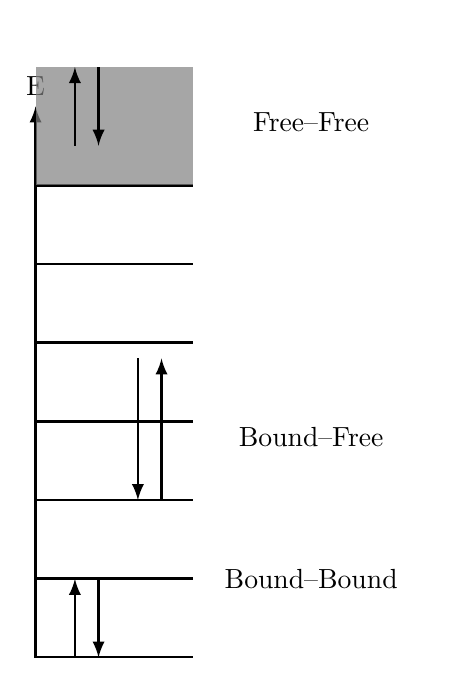
\begin{tikzpicture}[line width=1pt]
\clip (-0.1,0) rectangle +(5,8);
    \draw [-latex] (0,0) -- (0,7) node [above] {E};
\foreach \y in {0,\e1,\e2,\e3,\e4,\e5,\e6}
\draw (0,\y) -- (2,\y);
\fill [gray,opacity=0.7] (0,\e6) rectangle (2,\e6+1.5);
% Bound - Bound transition
\draw [-latex] (0.5,0) -- (0.5,\e1);
\draw [latex-] (0.8,0) -- (0.8,\e1);
\node at (3.5,1) {Bound--Bound};
% Free - Free transition
\draw [latex-] (0.5,\e6+1.5) -- +(0,-1);
\draw [-latex] (0.8,\e6+1.5) -- +(0,-1);
\node at (3.5,\e6+0.8) {Free--Free};
% Bound - Free transition
\draw [latex-] (1.3,\e2) -- +(0,1.8);
\draw [-latex] (1.6,\e2) -- +(0,1.8);
\node at (3.5,\e2+0.8) {Bound--Free};
\end{tikzpicture}
\end{document}
